%%%%%%%%%%%%%%
%% Run LaTeX on this file several times to get Table of Contents,
%% cross-references, and citations.

%% w-bktmpl.tex. Current Version: Feb 16, 2012
%%%%%%%%%%%%%%%%%%%%%%%%%%%%%%%%%%%%%%%%%%%%%%%%%%%%%%%%%%%%%%%%
%
%  Template file for
%  Wiley Book Style, Design No.: SD 001B, 7x10
%  Wiley Book Style, Design No.: SD 004B, 6x9
%
%  Prepared by Amy Hendrickson, TeXnology Inc.
%  http://www.texnology.com
%%%%%%%%%%%%%%%%%%%%%%%%%%%%%%%%%%%%%%%%%%%%%%%%%%%%%%%%%%%%%%%%

%%%%%%%%%%%%%%%%%%%%%%%%%%%%%%%%%%%%%%%%%%%%%%%%%%%%%%%%%%%%%%%%
\documentclass{wileysix}

\usepackage{w-bookps}
\usepackage{lipsum}
\usepackage{float}
\usepackage{graphicx}
\usepackage{color}
\usepackage{listings}

\begin{document}
\lstset{language=Python, breaklines=true, frame=T, keywordstyle=\color{blue}, morekeywords={*,self, not, None}, basicstyle=\footnotesize} 
	
\booktitle{Horno PID}
\subtitle{Electr\'onica para Ciencias}
\authors{Juan Barbosa\\
\affil{Departamento de F\'isica \\Universidad de los Andes}
Luisa Rodr\'iguez\\
\affil{Departamento de F\'isica \\Universidad de los Andes}
}

\halftitlepage
\titlepage


\offprintinfo{Horno PID}{Juan Barbosa}

\tableofcontents
\chapter{Controlador PID}

Con el objetivo de controlar la temperatura sobre un actuador, se realiza un circuito con controlador PID. El circuito en su totalidad se compone de 5 partes principales:
\begin{enumerate}
	\item \textbf{Sistema de alimentaci\'on:} tiene como objetivo generar los 5 V necesarios para encender la Raspberry Pi, as\'i como fijar el valor m\'aximo para la referencia.
	\item \textbf{Sensor de temperatura:} transforma la temperatura del actuador en una variable el\'ectrica que es medida por el controlador y mostrada al usuario en tiempo real. 
	\item \textbf{Valor de referencia:} corresponde con el valor de temperatura al que se desea llevar el accionador.
	\item \textbf{Controlador PID:} cont\'inuamente evalua la diferencia entre el valor de referencia y la temperatura actual, adem\'as de aplicar correci\'on que corresponden con t\'erminos proporcionales, integradores y derivativos.
	\item \textbf{Circuito de accionamiento:} tiene como objetivo proporcionar la potencia necesaria para que el actuador funcione de manera correcta.
\end{enumerate}

Estas partes se pueden observar en la Figura \ref{fig: circuito}, donde se dibuja el circuito usado para el horno PID. En ella cada parte se encuentra se\~nalada con un color espec\'ifico, siendo el sistema de alimentaci\'on, rojo; el sensor de temperatura, verde; el valor de referencia, azul; el controlador, naranja; y el circuito de accionamiento en violeta. 
\begin{figure}[h]
	\centering
	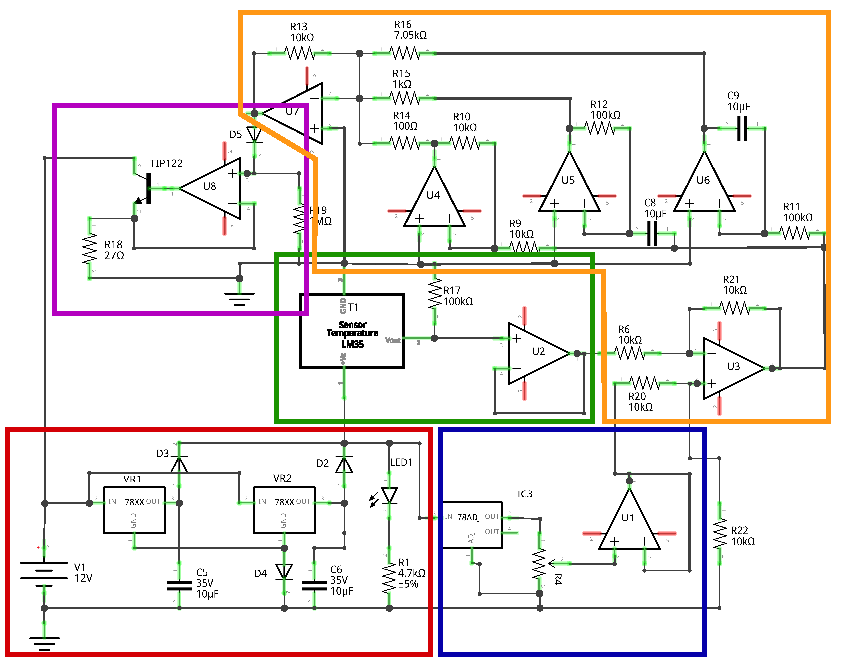
\includegraphics[width=\linewidth]{extras/circuit_schem.pdf}
	\caption{Circuito PID, implementado para el control de la temperatura.}
	\label{fig: circuito}
\end{figure}
\begin{figure}[h]
	\centering
	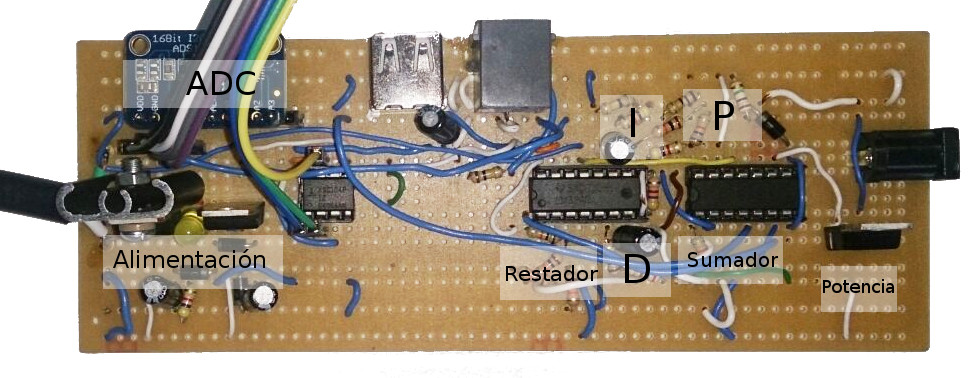
\includegraphics[width=\linewidth]{extras/circuit.jpg}
	\caption{Circuito implementado para el horno.}
\end{figure}

\section{Calibraci\'on de la temperatura}
El sensor de temperatura corresponde con un LM35, circuito integrado con respuesta lineal a la temperatura, con un factor de escala de 10 mV/$^\circ$C y un rango de operaci\'on de -55 $^\circ$C a 150 $^\circ$C \cite{LM35}. A pesar de ser un sensor calibrado, se realiza una calibraci\'on \textit{in situ} usando una termocupla de NiCr-Ni Phywe.
\begin{figure}[h]
	\centering
	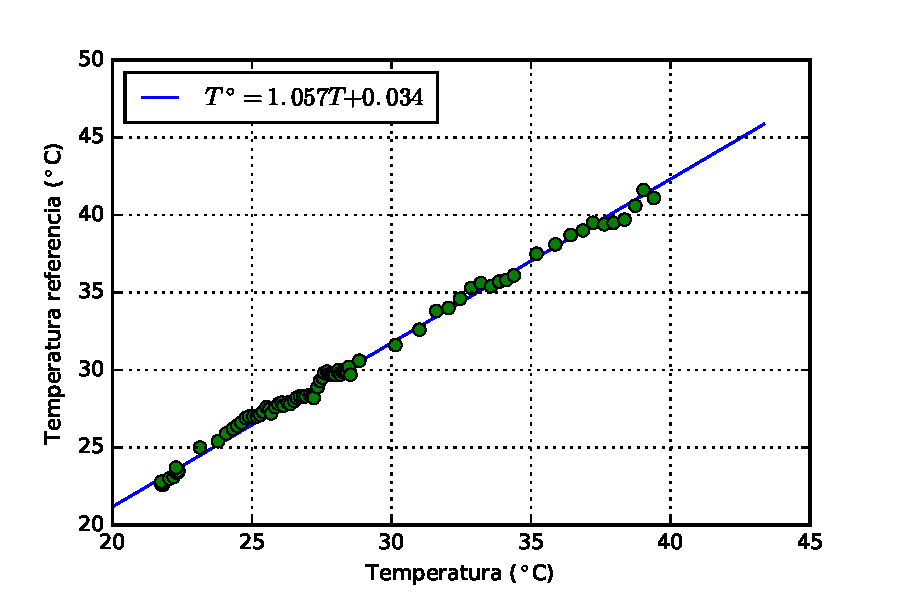
\includegraphics[width=0.7\linewidth]{extras/temp_cal.pdf}
	\caption{Calibraci\'on del sensor.}
	\label{fig: temp calibration}
\end{figure}

Los resultados se muestran en la Figura \ref{fig: temp calibration}, de donde se observa la linealidad del sensor usado, tanto la pendiente como el intercepto muestran desfases del valor esperado (1 y 0, correspondientemente) sobre la seg\'unda cifra decimal, discrepancias menores al 6 \%.

\section{Caracterizaci\'on del actuador}
Inicialmente la construcci\'on del horno usaba una celda Peltier, no obstante esta dej\'o de funcionar. Por este motivo se modifica el actuador a una resistencia de 27 $\Omega$ y 5 vatios. Para una resistencia la potencia es proporcional al cuadrado de la diferencia de potencial entre sus terminales:
\begin{equation}
	P = VI = V\left(\frac{V}{R}\right)
\end{equation}

\begin{figure}[h]
	\centering
	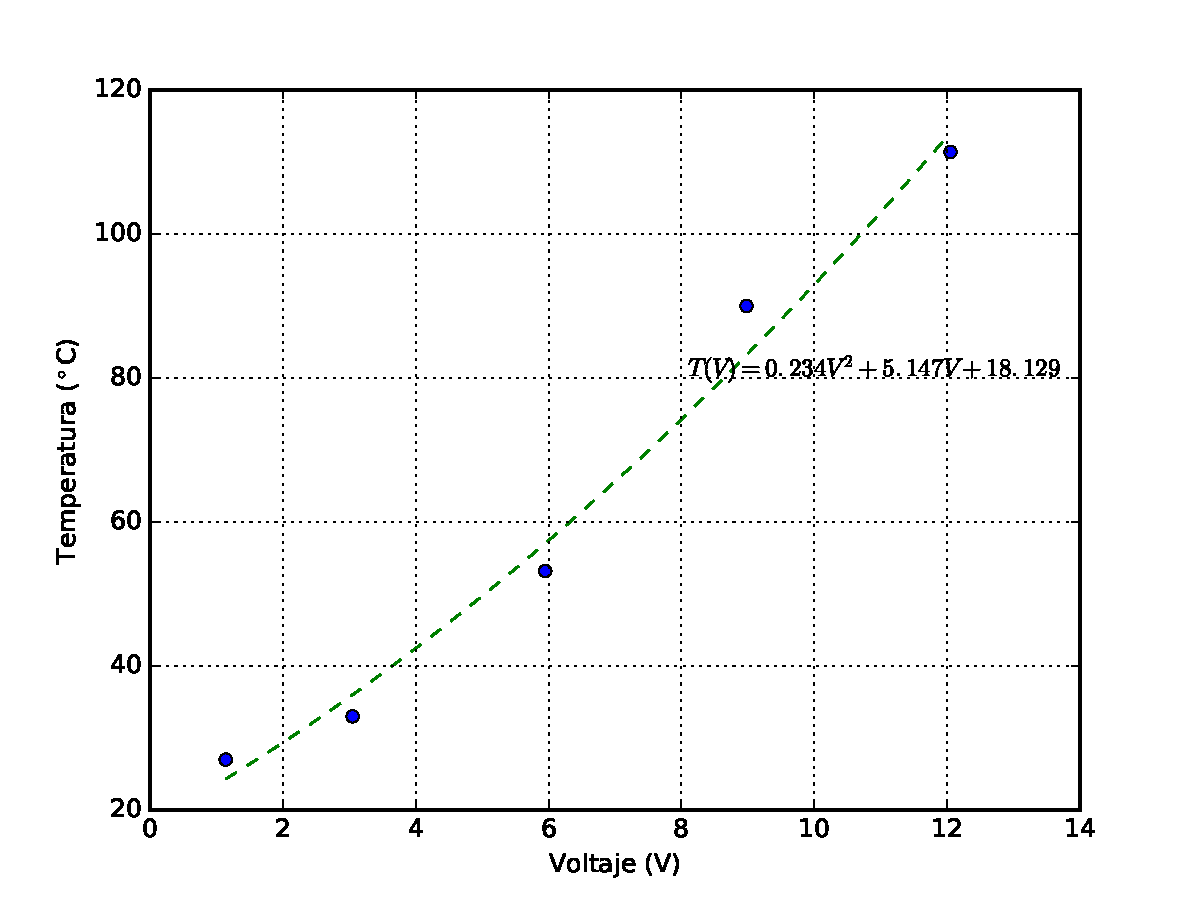
\includegraphics[width=0.7\linewidth]{extras/actuator.pdf}
	\caption{Temperaturas alcanzadas por la resistencia para distintos valores de voltaje.}
\end{figure}
Debido a que el sistema se encuentra restringido a voltajes de $\pm$12 y 0 V, la m\'axima potencia sobre la resistencia ser\'a 5.3 W, valor que se encuentra dentro de la capacidad de la resistencia.

\section{Sistema de alimentaci\'on}
El sistema de alimentaci\'on est\'a compuesto por dos reguladores de voltaje de 5 V de la familia 7805 \cite{7805}. El circuito de alimentaci\'on se encuentra acompa\~nado de dos condensadores que act\'uan como filtros, adem\'as se dispone de tres diodos 1N4001 \cite{1N4001} como protecci\'on a corriente reversa. El circuito sin carga mantiene un potencial de 5.03 V, y con carga se alcanzan valores de 4.78 V.
\begin{figure}[h]
	\centering
	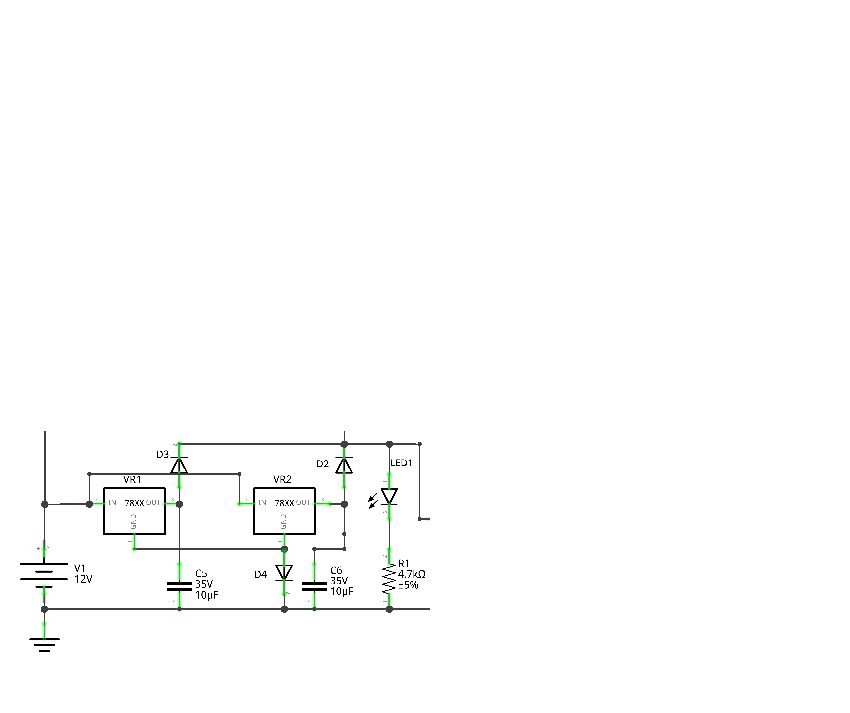
\includegraphics[width=0.9\linewidth]{extras/alimentacion.pdf}
	\caption{Circuito de alimentaci\'on del horno.}
\end{figure}

\section{Controlador}
El controlador est\'a compuesto por tres etapas:
\begin{itemize}
	\item \textbf{Restador:} calcula el error en la temperatura del horno.
	\item \textbf{PID:} todas las partes invierten la salida y mantienen la ganancia en 1.
	\item \textbf{Sumador:} se suma de forma ponderada las distintas componentes del PID. Las constantes usadas se muestran en la Tabla \ref{tb: PID}.
	
	\begin{table}[h]
		\centering
		\caption{Par\'ametros del controlador PID.}
		\begin{tabular}{|c|c|}
			\hline
			$K_P$ & 100 \\
			$K_I$ & 10 \\
			$K_D$ & 1.42 \\
			\hline
		\end{tabular}
		\label{tb: PID}
	\end{table}
\end{itemize}

Los par\'ametros del controlador fueron determinados manualmente. En primer lugar se determin\'o $K_P$ usando 8 valores distintos de $R_{13}$.
\begin{equation}
	K_P = \frac{R_{14}}{R_{13}}
\end{equation}

\begin{figure}[h]
	\centering
	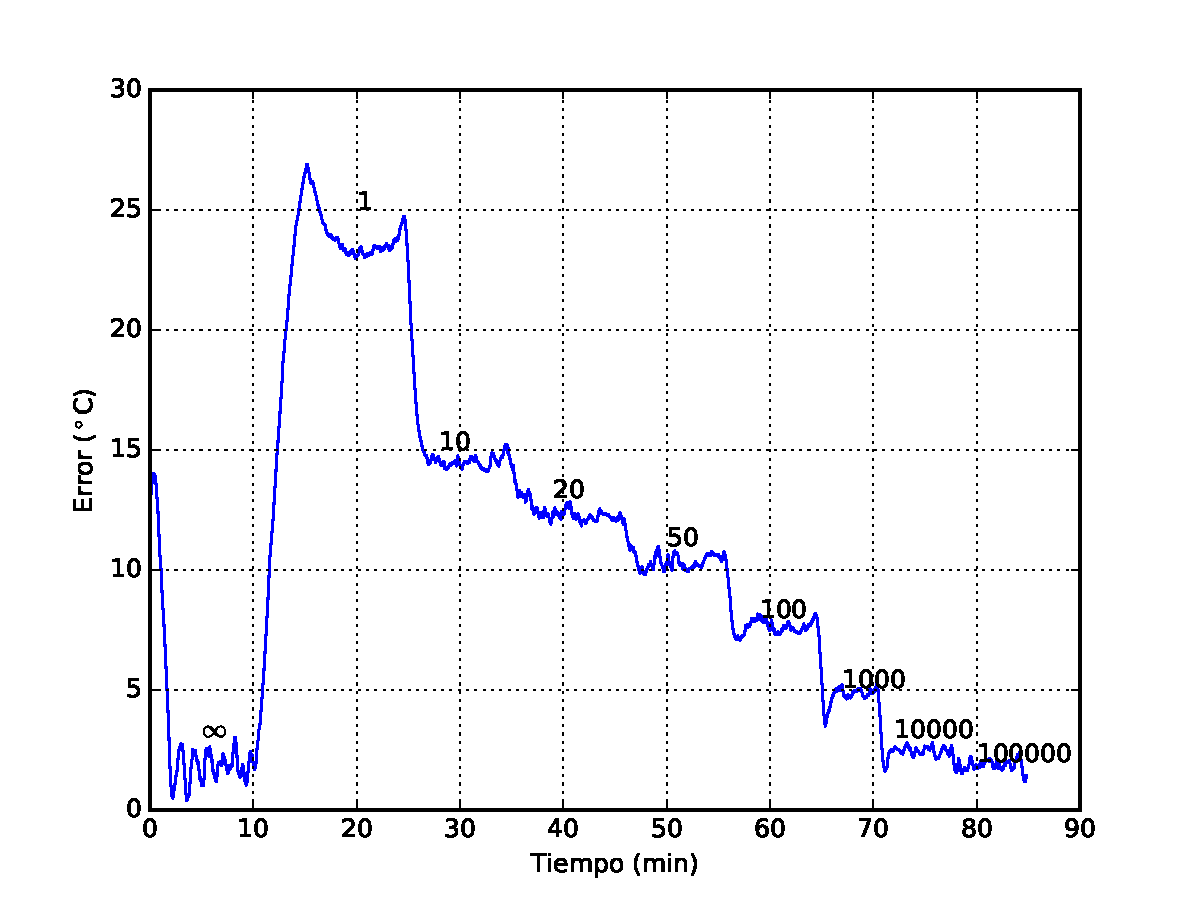
\includegraphics[width=0.6\linewidth]{extras/KP.pdf}
\end{figure}
En segundo lugar se agrega la etapa derivativa, para la cual la ganancia $K_D$ corresponde con;
\begin{equation}
	K_D = \frac{R_{14}}{R_{15}}
\end{equation}

\begin{figure}[h]
	\centering
	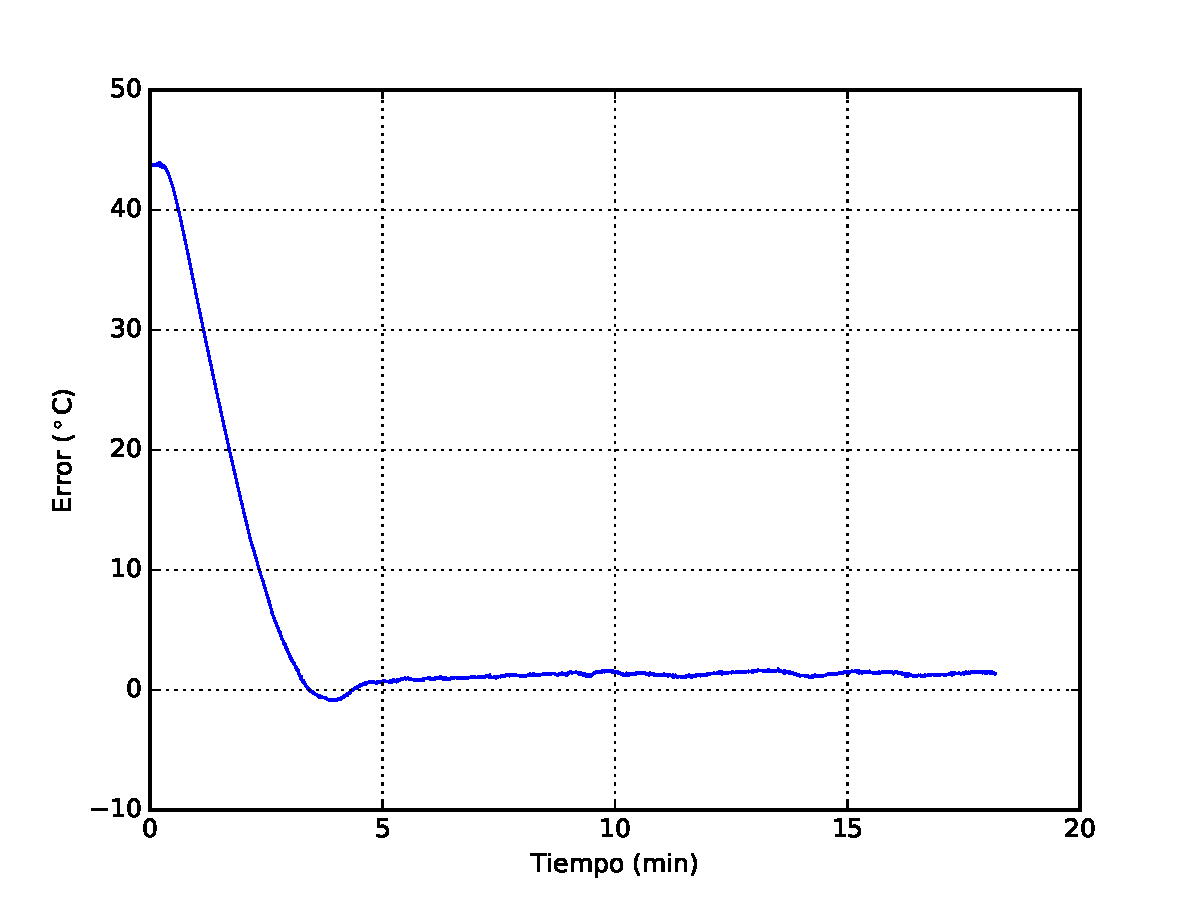
\includegraphics[width=0.6\linewidth]{extras/final_PID.pdf}
	\caption{Resultado final del controlador PID.}
\end{figure}
Finalmente se agrega una etapa integradora para eliminar el error del estado estacionario, los valores de $K_I$ con los que se prob\'o el circuito fueron: 10, 1 y 1.42. El primero, satura permanentemente el actuador, manteniendo siempre al m\'aximo la diferencia de potencial. Con el segundo se alcanza un error del estado estacionario para una temperatura de 67.6 $^\circ$C en 3 $^\circ$C, error que se reduce con la \'ultima constante a cerca de 1 $^\circ$C.

\section{Digitalizaci\'on}
El valor de referencia es fijado usando un potenciometro digital con referencia X9C103P \cite{digi-pot} con resistencia interna de 100 k$\Omega$. Los tres pines l\'ogicos son conectados a los GPIO, los puertos predeterminados son:
\begin{enumerate}
	\item[19] \textbf{IN} (INCREMENT) 
	\item[20] \textbf{U/D} (UP/DOWN)
	\item[21] \textbf{C/S} (CHIP SELECT)
\end{enumerate}

Sin embargo los mismos pueden ser modificados usando la interf\'az gr\'afica. A continuaci\'on se muestran dos curvas del potencial en funci\'on de la posici\'on de la aguja del potenci\'ometro.
\begin{figure}[h]
	\begin{tabular}{cc}
		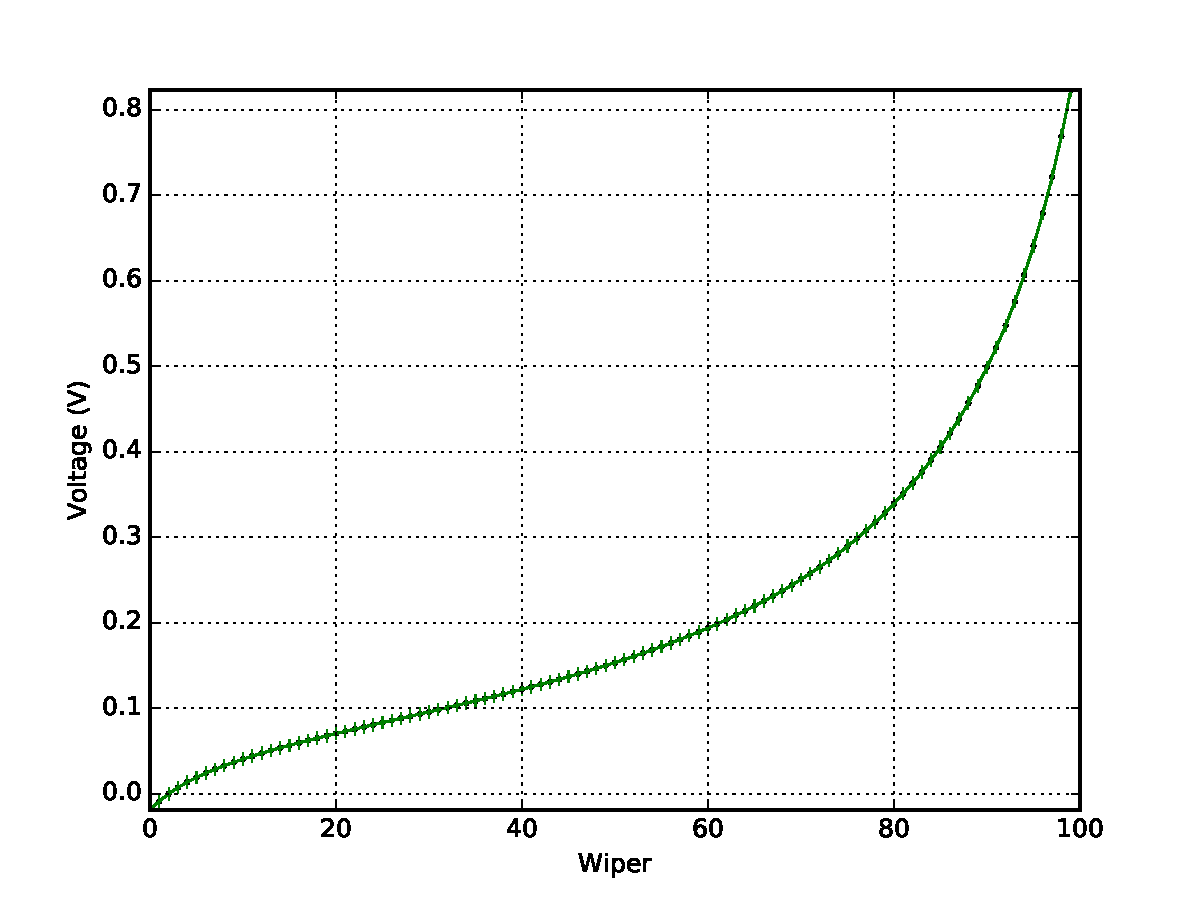
\includegraphics[width=0.5\linewidth]{extras/without_follower.pdf}
		& 
		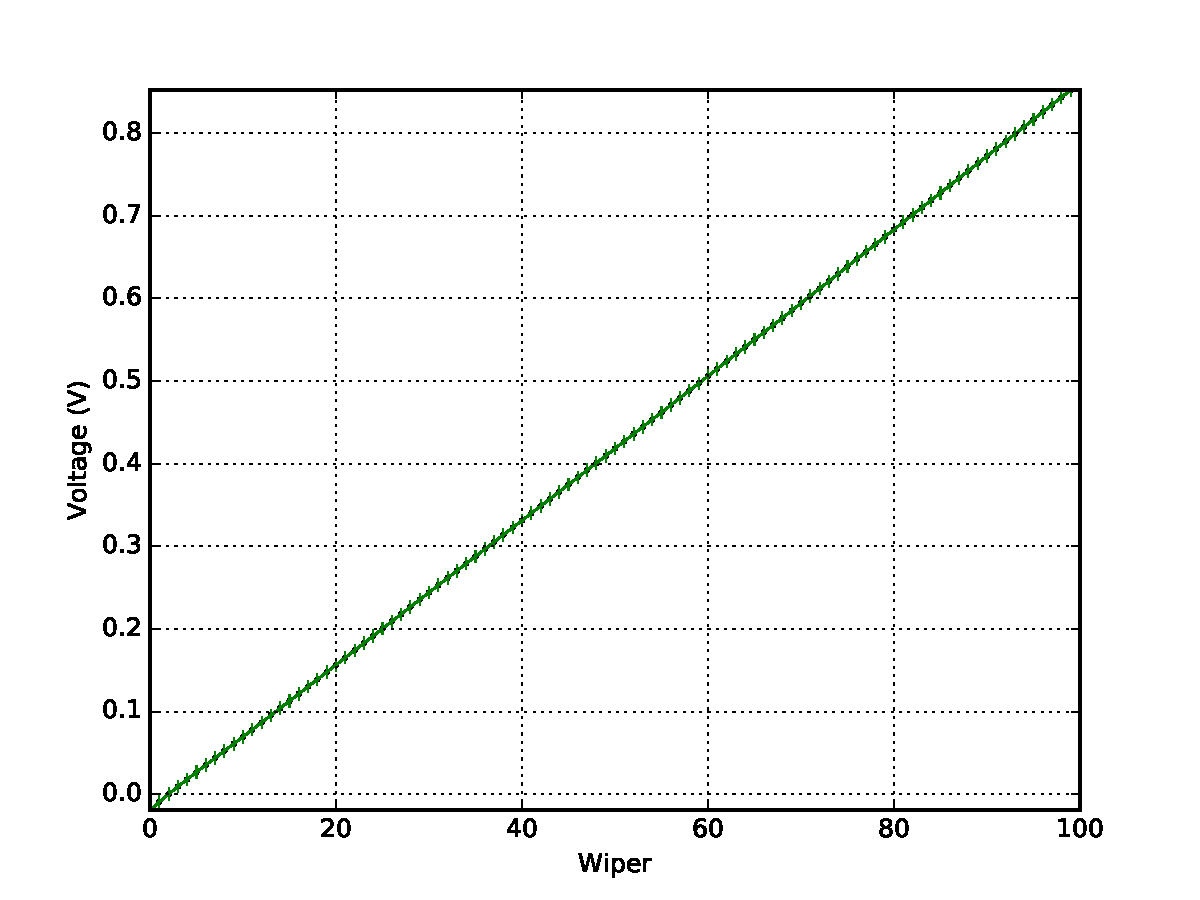
\includegraphics[width=0.5\linewidth]{extras/with_follower.pdf}
	\end{tabular}
	\caption{Voltaje de salida del potenci\'ometro acoplado al restador del PID. A la izquierda con carga, en el derecho con seguidor.}
\end{figure}

En las figuras anteriores se puede apreciar el efecto de la carga sobre el divisor de voltaje. Una modificaci\'on final en la etapa de digitalizaci\'on permiti\'o lograr un rango de potenciales de 0 a 3.3 V, conservando la linealidad, pero reduciendo la selecci\'on de temperaturas a cada 3.3 $^\circ$C.

\begin{figure}[h]
	\centering
	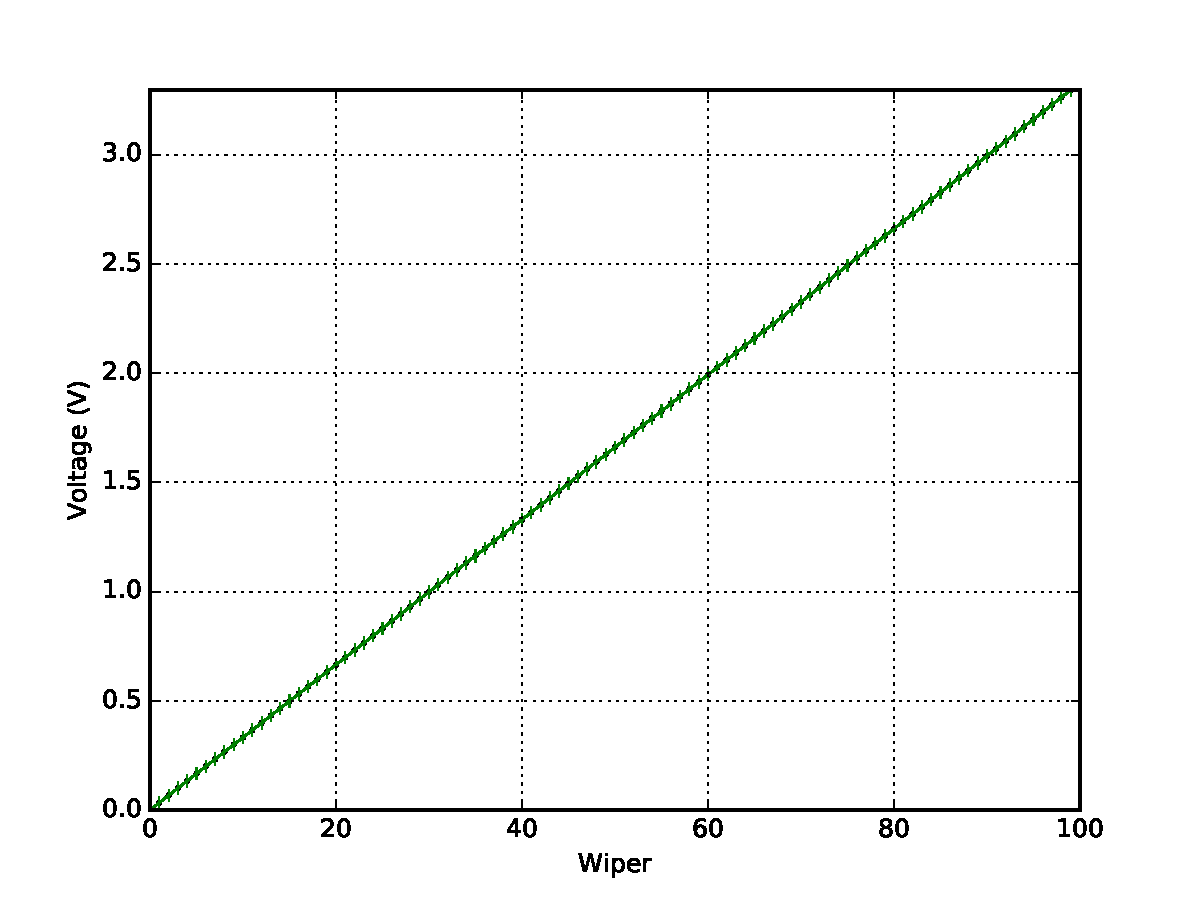
\includegraphics[width=0.7\linewidth]{extras/final_cal.pdf}
	\caption{Calibraci\'on final del potenciometro digital.}
\end{figure}
\begin{chapreferences}{10.}
	\bibitem{LM35} Texas Instruments, ``LM35 Precision	Centigrade Temperature Sensors'' LM35 datasheet, Aug. 1999 [Revised Aug.
	2016].
	\bibitem{7805} Spark fun ``Positive-Voltage Regulators'' $\mu$A7805C datasheet, May. 1976 [Revised May. 2003].
	\bibitem{1N4001} Diodes, ``Diffused Junction 1N4001 - 1N4007'' 1N4001 datasheet, Sep. 2004.
	\bibitem{digi-pot}
	Digitally Controlled Potentiometer ``X9C103'' datasheet, Jul 2009.
\end{chapreferences}

\chapter{Algoritmo}
\begin{figure}[h]
	\centering
	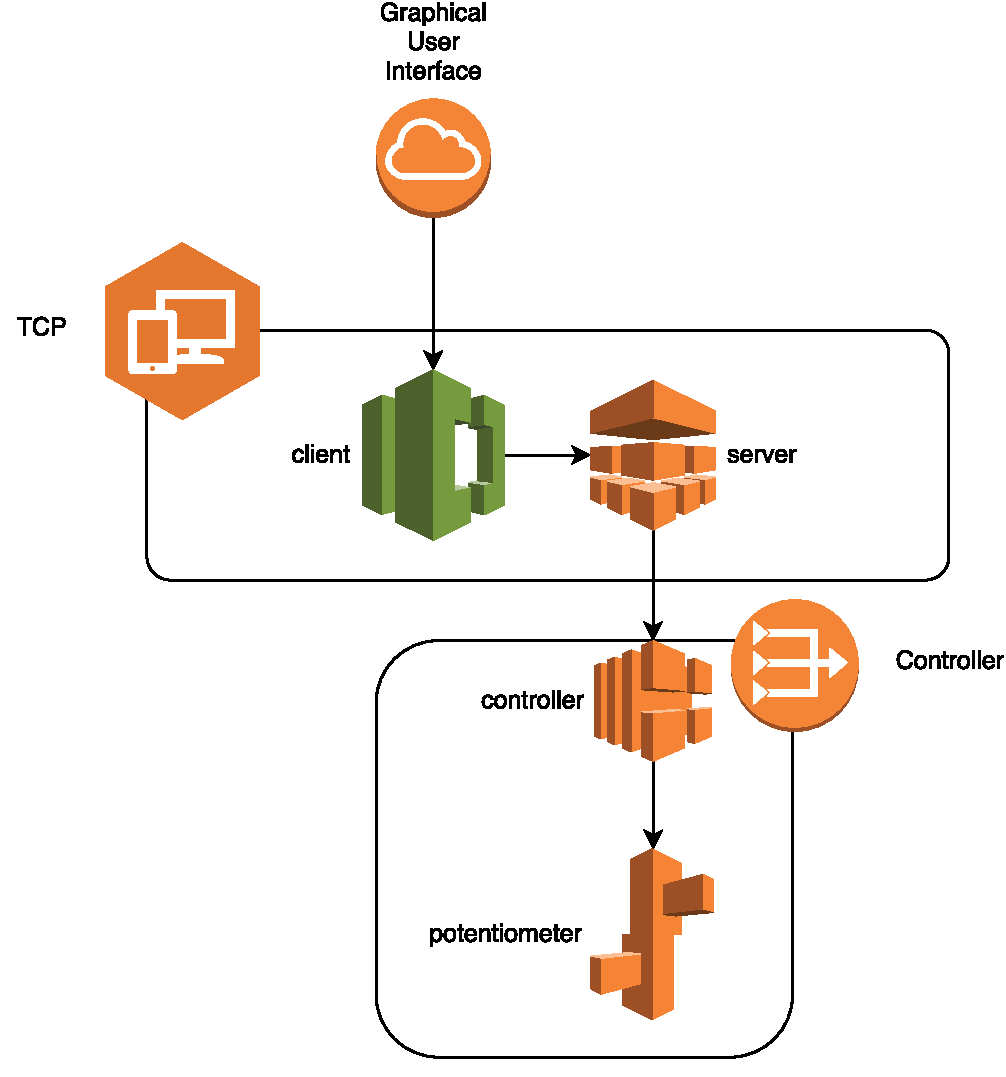
\includegraphics[width=0.5\linewidth]{extras/diagram.pdf}
	\caption{Jerarqu\'ia de las clases usadas por la interfaz gr\'afica.}
	\label{fig: diagram}
\end{figure}
\pagebreak

La parte computacional del proyecto est\'a escrita en su totalidad en Python y usa una interfaz gr\'afica en Qt. Usando un paradigma de programaci\'on por objetos fueron creadas 5 clases que siguen la jerarqu\'ia que se muestra en la Figura \ref{fig: diagram}. 

\section{peltier.py}
Contiene la informaci\'on relacionada con la interfaz gr\'afica, configura las se\~nales y puertos necesarios por los objetos propios de Qt.
\lstinputlisting{extras/peltier.py}

\section{TCP.py}
Contiene las clases \verb|client| y \verb|server| que funcionan como cliente y servidor TCP (Protocolo de Control de Transmisi\'on) los cuales permanentemente intercambian los datos de temperatura deseada, actual y referencia. El uso de un servidor TCP permite interactuar con el horno a trav\'es de una red LAN.
\lstinputlisting{extras/TCP.py}

\section{controller.py}
Contiene las clases \verb|controller| y \verb|potentiometer|, la primera determina los puertos l\'ogicos con los que la Raspberry controla el potenciometro digital, adem\'as, determina la posici\'on de la aguja del potenciometro para la cual se obtiene el voltaje m\'as cercano a la temperatura deseada. La clase \verb|potentiometer| est\'a en capacidad de modificar la posici\'on de la aguja del potenciometro cada vez que \verb|controller| lo considere necesario.
\lstinputlisting{extras/controller.py}

\newpage
Los c\'odigos del proyecto as\'i como los datos obtenidos para las curvas de calibraci\'on se encuentran publicados en GitHub, y hacen parte del repositorio \verb|supreme-pi| como parte de un proyecto de \textit{physical computing} \cite{GitHub}.
\begin{chapreferences}{10.}
	\bibitem{GitHub}
	B. Juan, \textit{supreme-pi}, GitHub repository,
	https://github.com/jsbarbosa/supreme-pi
\end{chapreferences}

\chapter{Mejoras}
Las mejoras al sistema de control se centran en los par\'ametros del PID. En ese sentido se considera que la mayor mejora se encuentra en la aplicaci\'on de algoritmos que permitan determinar los valores ideales midiendo iterativamente la respuesta del sistema para distintos valores de $K_P$, $K_I$ y $K_D$.

Es necesario tener en cuenta que la familia de potenciometros usados X9Cxxx solo pueden tener una diferencia de potencial entre $\pm$5 V y 0 V entre las terminales de la resistencia, raz\'on por la cual es necesario recurrir a otras referencias de potenciometros digitales que no tengan esta limitante.
\end{document}